\chapter{Introduccion}
\label{capitulo1}
\lhead{Capítulo 1. \emph{Introduccion}}
% De qué va a tratar el capítulo

La navegación y exploración en áreas de difícil acceso mediante el uso de robots, es una tarea que se ha venido desarrollando en el Grupo de Investigación y Desarrollo en Mecatrónica de la USB  \textit{(GIDM)} desde hace mu tiempo. Donde una de las aplicaciones mas demandantes, es la tarea de reconstruir un mapa 2D de la superficie mapeada por los robots utilizados. En el presente capitulo se pretende introducir los trabajos previos y avances que se han tenido en el desarrollo de este tipo aplicaciones, tanto en el \textit{GIDM} como a nivel mundial, y que dieron origen y motivación para la realización del proyecto. Además, de postular un serie de problemas que el presente trabajo busca solucionar.

\section{Antecedentes}

Cuando se habla de construir un mosaico 2D, se hace referencia al proceso de recortar y alinear imágenes, de tal forma que puedan ser representadas todas juntas en una sola gran imagen. Es importante considerar que las imágenes para este tipo de aplicaciones son capturadas desde diferentes ubicaciones de la cámara, a diferencia del proceso para elaborar imágenes panorámicas, en las cuales esta ubicación es una constante. 

La elaboración de mosaicos para la construcción de mapas del suelo, se ha desarrollado incluso antes desde la era digital de la computadoras. Desde que el proceso de registrar fotografías ha existido, se comenzaron a usar para elaborar mapas topográficos \cite{primeros-mapas}, donde imágenes adquiridas a partir de globos aerostáticos o altas colinas eran unidas manualmente. Posteriormente, producto de los avances en materia de aeronáutica, el interés por la aerofotografía se incrementó en gran medida. En este mismo sentido se utilizaban aviones para el registro de imágenes a mayores altitudes, y se cubrían mayores áreas en menor cantidad de tiempo, pero debido a que no se alcanzaban alturas tan altas, y se mantenía la necesidad de registrar grandes áreas, era requerido que los mapas se construyan mediante fotografías que se superpongan, de igual forma esta tarea se llevaba a cabo mediante técnicas manuales por medio de expertos.

La necesidad de registrar áreas aun mas grandes siguió avanzando, motivado por la llegada de los satélites que eran capaces de enviar a tierra la información que obtenían de las cámaras. Los avances tecnológicos en materia de computación, y el creciente aumento de datos para esta aplicación, promovieron el desarrollo de técnicas de procesamiento digital de imágenes para dar solución a este tipo de problemas.

Del mismo modo, distintos centros de investigación en el área de la física, robótica y visión por computadora, han aplicados sus esfuerzos en desarrollar algoritmos para la realización de estos mapas en ambientes mas desafiantes como lo son el fondo marino \cite{gracias-victor,Pizarro-singh,eustice,Allais}. Cuando se opera en este tipo de ambientes, en busca de realizar exploraciones mas eficientes y a mayor escala, se emplean vehículos operados remotamente \textit{ROV} (del inglés: Remotely Operated Vehicles) o vehículos autónomos submarinos \textit{AUV} (del inglés: Automated Underwater Vehicles). 

\section{Justificación y planteamiento del problema}

En el \textit{GIDM} se han realizado grandes avances en el desarrollo de equipos y plataformas robóticas, específicamente para su uso en aplicaciones submarinas. En este sentido, se cuenta con un vehículo submarino llamado OpenROV\footnote{\url{https://www.openrov.com/products/openrov28/}}, el cual se puede apreciar en la figura \ref{imagen:openrov}. OpenROV es un robot operado remotamente de baja albergadura diseñado especialmente para operar bajo el agua.

\begin{figure}[H]
	\centering
	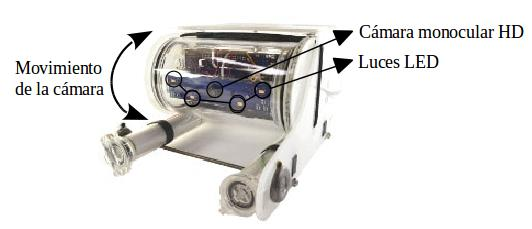
\includegraphics[width=0.7\textwidth]{openrov}
	\caption{Robot móvil OpenROV}
	\label{imagen:openrov}
\end{figure}

\begin{wrapfigure}{r}{0.3\textwidth}
	\begin{center}
		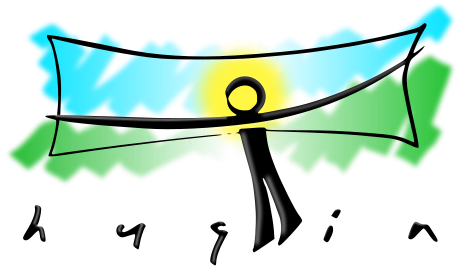
\includegraphics[width=0.3\textwidth]{hugin}
	\end{center}
	\caption{Logo del software Hugin}
\end{wrapfigure}

En el \textit{GIDM} actualmente se utilizan mecanismos manuales para la elaboración de estos mapas, en especifico, se hace uso de \textit{softwares} como Hugin\footnote{\url{hugin.sourceforge.net/}}. Este es un programa de código abierto y gratuito bajo licencia GPL\footnote{\url{http://www.gnu.org/copyleft/gpl.html}}, el cual esta dedicado a la generación de imágenes panorámicas, incluyendo funciones para el recorte, alineación, corrección de color; además de algoritmos para la optimización de parámetros en la cámara, y corrección de distorsión. Si bien este software esta diseñado para la creación de imágenes panorámicas, permite el uso de varios tipos de proyecciones cartográficas, entre estas la rectangular, proyectando las imágenes sobre un plano recto.

    
Atendiendo a esta necesidad, es necesario contar con un sistema que permita realizar la reconstrucción del suelo con la menor interacción posible del ser humano. Asimismo, con el fin de poder realizar operaciones de mapeo y localización simultanea \textit{SLAM}, haciendo uso de las herramientas y robots existentes en el laboratorio, es necesario contar con un sistema basado en visión, que genere de forma automática un mapa 2D de la superficie sobre la que navega o sobrevuela el vehículo remoto.


\section{Objetivos}

\subsection{Objetivo General}

Analizar e implementar un sistema automatizado que permita la reconstruccion de un mapa en dos dimensiones, del entorno recorrido por robot, aereo o submarino.

\subsection{Objetivos Específicos}

\begin{itemize}
	\item Análisis comparativo de metodos vigentes en la reconstruccion de mosaicos 2D, a partir de imagenes y videos de entrada.
	\item Implementacion de modulo de preprocesamiento y correccion de entrada.
	\item Analisis comparativo de metodos de deteccion y description de puntos clave.
	\item Implementación de módulo de alineación de imagenes mediante la deteción de puntos clave.
	\item Cuantificar el error de reproyeccion y distorsion en los modelos 2D generados.
\end{itemize}

\section{Estructura del trabajo}

Luego de presentar el planteamiento del problema y la descripción del proyecto, la presente investigación se encuentra dividida en 5 capítulos, organizados de la siguiente manera:

En el \textit{\textbf{Capitulo 2}} se presenta una revisión del estado del arte sobre los algoritmos de generación de mosaico, en el cual se exponen los trabajos recientes y avances importantes en esta área de investigación. En ese mismo sentido, se describen los módulos principales que componen este tipo de sistemas.

El \textit{\textbf{Capitulo 3}} comprende una revisión teórica en la cual se describe el funcionamiento de los algoritmos detectores, descriptores y emparejadores de características, así como también resultados de pruebas comparativas entre los mas usados para este tipo de aplicaciones. 

El módulo encargado de la alineación de imágenes en el mosaico es descrito en el \textit{\textbf{Capitulo 4}}. Al igual que el capitulo anterior, se presenta una revisión teórica de los conceptos necesarios para su implementación. Luego, se introduce el modelo de sub mosaicos, y la implementación de un conjunto de correcciones geométricas sobre este nuevo modelo. Finalmente se presentan los resultados de los algoritmos aplicados en esta sección, seguidos de sus respectivos análisis.

En el \textit{\textbf{Capitulo 5}} se describe el modulo final del sistema, en donde se explica el funcionamiento de los algoritmos que corrigen visualmente el mosaico final. De igual forma se muestran los resultados de su implementación, seguidos de una conclusión final sobre estos.

Finalmente, en el \textit{\textbf{Capitulo 6}} se presentan las conclusiones finales, además de propuestas sobre posibles implementaciones y recomendaciones que pueden aportar mejoras y/o permitir la continuación del proyecto aquí planteado.